\documentclass[a4paper,11pt]{article}

\setlength{\parindent}{0cm}
\setlength{\parskip}{9pt}
\usepackage[margin=2cm]{geometry}

\usepackage{amsmath,amssymb,graphicx}
\title{\textsc{CELEN087 - Lecture Four}}
\author{Aidin Jalilzadeh}
\date{\today}

\begin{document}

\maketitle

\section{Mathematics - Cases}

The absolute value function $f(x)=|x|$ is defined as:

\begin{equation*}
|x|=
\begin{cases}
x & \textrm{if} \quad x \geq 0 \\
-x & \textrm{if} \quad x \leq 0
\end{cases}
\end{equation*}

\section{Table}
Here is a table of fruits and their colours and prices in RMB shown in Table \ref{T1}.

\begin{table}[h]
\centering
\begin{tabular}{|l|r|c|}
\hline
Fruit & Colour & Price (RMB) \\
\hline
\hline
Apple & Green & 10 \\
\hline
Grapes & Blue & 50\\
\hline
Strawberries & Red & 35\\
\hline
Mango & Yellow & 25\\
\hline
\end{tabular}
\caption{Fruits, colours and prices}
\label{T1}
\end{table}

\newpage
\section{Including Figures}

Here is a picture I am including in Figure \ref{EU}. 

\begin{figure}[t]
\centering
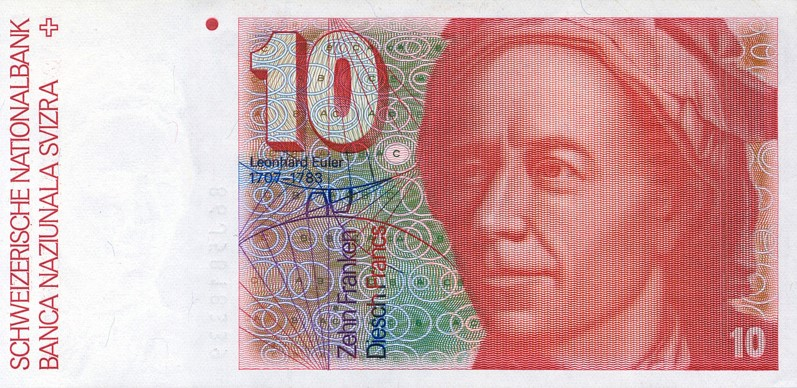
\includegraphics[scale=0.75]{Euler}
\caption{This is Euler}
\label{EU}
\end{figure}

\section{Numbered Lists}

This is a numbered list with three items:
\begin{enumerate}
\item Algorithms
\item Programming
\item Mathematical softwares
\item \LaTeX
\end{enumerate}


\section{Bullet-Point Lists}

This is a bullet-point list with three items:
\begin{itemize}
\item[(i)] Algorithms
\item[(ii)] Programming
\item[(iii)] Mathematical softwares
\item[(iv)] \LaTeX
\end{itemize}


















\end{document}